\section{Motivation}\label{sec:motivation}

It is well known that router administrative interfaces present an attack surface, allowing attackers to scan for vulnerabilities and reconfigure the router through malicious requests~\cite{niemietz2015owning,jeitner2022xdri}.
Unlike in a terrestrial setting, a satellite router is often part of a physical system including a motorized dish which can be affected.
Since these networks are in remote locations and contain many untrusted users, one bad actor can deny service to many users.

Despite these issues, new routers are being implemented without the institutional memory of historic vulnerabilities and their mitigations.
Alongside traditional router interface attacks, this opens up new denial of service through the physical system: rotating the dish and overusing the motor.

In this poster we summarize the key findings of most recent work which assesses the security of the Starlink user terminal~\cite{dishing-out-dos}.
We pay particular attention to the attack surface exposed by its web admin interface.
We explore both how configuration requests are made and the effects of sending undocumented commands, using a fuzzer to iterate through the unauthenticated command space.
We find an exploit in the command decoding and execution logic which, when combined with commands affecting the physical state of the dish, result in denial of service persisting until the router is physically power-cycled.
This can be widely exploited due to poor security practices such as a lack of password authentication on the admin interface, and default passwords on the WiFi network itself.

After disclosure, Starlink mitigated this issue in December 2022 in patch \textit{8c03f1b9-de75-404b-87fd-7986892cdacb.uterm.release}.


\begin{figure}
    \centering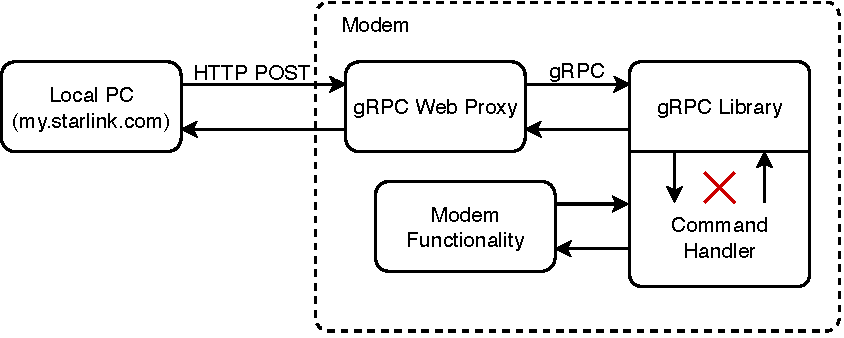
\includegraphics[width=\columnwidth]{img/modem.pdf}
    \caption{Overview of the Starlink modem functionality. gRPC calls, encapsulated within HTTP POST requests, are decoded and processed. Malformed requests cause the command handler to crash, resulting in the modem no longer being able to respond to commands.}
    \label{fig:modem}
    \vspace{-1em}
\end{figure}
